\iffalse
\documentclass[a4paper,12pt,twocolumn]{article}
\usepackage{graphicx}
\usepackage[margin=0.5in]{geometry}
\usepackage[cmex10]{amsmath}
\usepackage{array}
\usepackage{gensymb}
\usepackage{booktabs}
\title{Circle Assignment}

\author{Ravi Sumanth Muppana- FWC22003}
\date{September 2022}
\providecommand{\norm}[1]{\left\lVert#1\right\rVert}
\providecommand{\abs}[1]{\left\vert#1\right\vert}
\let\vec\mathbf
\newcommand{\myvec}[1]{\ensuremath{\begin{pmatrix}#1\end{pmatrix}}}	
\newcommand{\mydet}[1]{\ensuremath{\begin{vmatrix}#1\end{vmatrix}}}
\providecommand{\brak}[1]{\ensuremath{\left((#1\right)}}
\begin{document}
\maketitle
\section{Problem:}
<<<<<<< HEAD
A quadrilateral $ABCD$ is drawn to circumscribe a circle. Show that $\vec{AB+CD}$ is equal to $\vec{BC+AD}$
=======
\fi
A quadrilateral $ABCD$ is drawn to circumscribe a circle. Show that $AB+CD$ is equal to $BC+AD$
	\begin{figure}[!h]
		\centering
 \includegraphics[width=\columnwidth]{chapters/10/10/2/8/figs/circle.png}
		\caption{}
		\label{fig:10/10/2/8}
  	\end{figure}
	\\
	\solution 
	\begin{enumerate}
		\item  Draw the circle.
		\item Choose the point $\vec{A}$.
		\item Draw the tangents from $\vec{A}$ to the circle.
		\item Choose points $\vec{B}, \vec{D}$ on the tangents.
		\item From $\vec{B}, \vec{D}$, draw tangents to the circle intersecting at $\vec{C}$.
	\end{enumerate}
\iffalse
>>>>>>> f531642 (Created codes and figs folder)
\maketitle
\section{Solution:}
\begin{figure}[h]
	\includegraphics[width=\linewidth]{circle.png}
	\caption{Circle}
\end{figure}
\subsection{Theory:}
The sides of quadrilateral act as tangents to the circle. Also, the tangents at any point is at right angle to the radius of the circle. Let us assume two vectors $\vec{a}$ and $\vec{b}$.
\subsection{Mathematical Calculation:}
The possible tangents to the circle w.r.t vertices are (AP,AQ,BQ,BR,CR,CS,DS,DP). Let us consider the tangents AP,AQ. Their addition vector is $\vec{X}$. The radius of the circle be $\vec{y}$.
\begin{align*}
<<<<<<< HEAD
&\vec{P-A} = \vec{a}\\
&\vec{Q-A} = \vec{b}\\
	&\vec{O-P} = \vec{O-Q} = \vec{y}\\
=======
&\vec{P-A}\\
&\vec{Q-A}\\
	&\vec{O-P} = \vec{O-Q}\\
>>>>>>> f531642 (Created codes and figs folder)
\end{align*}
In triangle APO and AQO,  
\begin{align*}
	&\vec{O-A}= \vec{(O-P)+(P-A)}\\
	&\vec{O-A}= \vec{(O-Q)+(Q-A)}\\
<<<<<<< HEAD
&||\vec{O-A}||^2 = ||\vec{y+a}||^2\\
	&||\vec{O-A}||^2 = ||\vec{y+b}||^2\\
	&||\vec{O-A}||^2 = ||\vec{y}||^2 +2(\vec{y^Ta}) +||\vec{a}||^2\\
&||\vec{O-A}||^2 = ||\vec{y}||^2 +2(\vec{y^Tb}) +||\vec{b}||^2\\
\end{align*}
As $\vec{(y,a)}$ and $\vec{(y,b)}$ are perpendicular to each other, the terms $+2(\vec{y^Ta})$ and $+2(\vec{y^Tb})$ will be equal to zero. 
\begin{align*}
&||\vec{O-A}||^2 = ||\vec{y}||^2 + ||\vec{a}||^2 \\
&||\vec{O-A}||^2 = ||\vec{y}||^2 + ||\vec{b}||^2\\
&||\vec{a}|| = ||\vec{b}||
=======
	&||\vec{O-A}||^2 = ||\vec{(O-P)+(P-A)}||^2\\
	&||\vec{O-A}||^2 = ||\vec{(O-Q)+(Q-A)}||^2\\
	&||\vec{O-A}||^2 = ||\vec{O-P}||^2 +2(\vec{(O-P)^T(P-A)})\\ +||\vec{P-A}||^2\\
	&||\vec{O-A}||^2 = ||\vec{O-Q}||^2 +2(\vec{(O-Q)^T(Q-A)})\\ +||\vec{Q-A}||^2\\
\end{align*}
As $\vec{(O-P),(P-A)}$ and $\vec{(O-Q),(Q-A)}$ are perpendicular to each other, the terms $+2(\vec{(O-P)^T(P-A)})$ and $+2(\vec{(O-Q)^T(Q-A)})$ will be equal to zero. 
\begin{align*}
&||\vec{O-A}||^2 = ||\vec{O-P}||^2 + ||\vec{P-A}||^2 \\
&||\vec{O-A}||^2 = ||\vec{O-Q}||^2 + ||\vec{Q-A}||^2\\
	&||\vec{P-A}|| = ||\vec{Q-A}||
>>>>>>> f531642 (Created codes and figs folder)
\end{align*}
Therefore, the lengths AP is equal to AQ.\\
Similarly, if we take the rest of the tangents as vectors and solve in the same way, we get $BR = BQ$, $CR = CS$, $DP = DS$.
Now, add all the above equations and we get,
\begin{align*}
<<<<<<< HEAD
	&\vec{(AP+BR+CR+DP)} = \vec{(AQ+BQ+CS+DS)}\\
	&\vec{(AD+BC)} = \vec{(AB+CD)}
=======
	&(AP+BR+CR+DP) = (AQ+BQ+CS+DS)\\
	&(AD+BC) = (AB+CD)\\
>>>>>>> f531642 (Created codes and figs folder)
\end{align*}
Hence proved.
\section{Construction:}
The construction of rhombus can be done using only two diagonals, taken as d1 and d2.
\begin{table}
	\centering
\setlength\extrarowheight{2pt}
	\begin{tabular}{|c|c|c|}
		\hline
		\textbf{vertices, variables} & \textbf{formulae} & \textbf{Comments}\\
		\hline
<<<<<<< HEAD
		(a,c,d,r) & (8,3,4,5) & ;sides and radius\\
		\hline
		theta1 & 2*mp.atan(r/d) & angle ADC\\
		\hline
		theta2 & 2*mp.atan(r/a) & angle BAD\\
		\hline                   
		theta3 & 2*mp.atan(r/c) & angle BCD\\
		\hline
		D & (0,0) & vertex D\\
		\hline
		O & (d,r) & centre O\\
		\hline
		C & (c+d)*e1& e1 = (1,0), direction vector\\
		\hline
		A & (a+d)*[(mp.cos(theta1),mp.sin(theta1)] & vertex A\\
		\hline
		m1 & [1, mp.tan(theta1+theta2)] & directional vector\\
		\hline
		B  &  A+lam[0]*m1 & lam = LA.solve(matM,C-A)\\
=======
		O & (1.414,0) & Center\\
		\hline
		r & 1 & radius\\
		\hline
		R & r+d & vertex dist.\\
		\hline
		theta & 270(pi/360) & vertex angle\\
		\hline
		delta1 & 2 & intrsctn dist frm vertex\\
		\hline
		delta2 & 3 & intrsctn dist frm vertex\\
>>>>>>> f531642 (Created codes and figs folder)
		\hline
	\end{tabular}
\end{table}

\end{document}
\fi
